% \documentclass[9pt]{article}
\documentclass[9pt,a4]{article}
\usepackage[9pt,inchmargins]{sigmin}

\usepackage{graphics}
\usepackage{epsfig}
\usepackage{xspace}
\usepackage[nolineno,noindent,norules]{lgrind}
\usepackage{subfig,graphics,graphicx,color}
\DeclareGraphicsExtensions{.eps}

%% Reference stuff.
\usepackage[square,comma,numbers,sort]{natbib}
\usepackage{hypernat}
\usepackage{hyperref}
\hypersetup{
  colorlinks=false,
  pdfborder={0 0 0},
  %pdftitle={\mytitle},
  %pdfkeywords={\mykeywords},
  bookmarksnumbered,
  pdfstartview={FitH},
  urlcolor=cyan,
  pdfpagelabels=true,
  pdfdisplaydoctitle=true,
}

% \renewcommand*{\bibfont}{\scriptsize}
\begin{document}

\textbf{Appendix (C): Non-text figures}
\vspace{0.3in}

\begin{figure}[h]
   \center
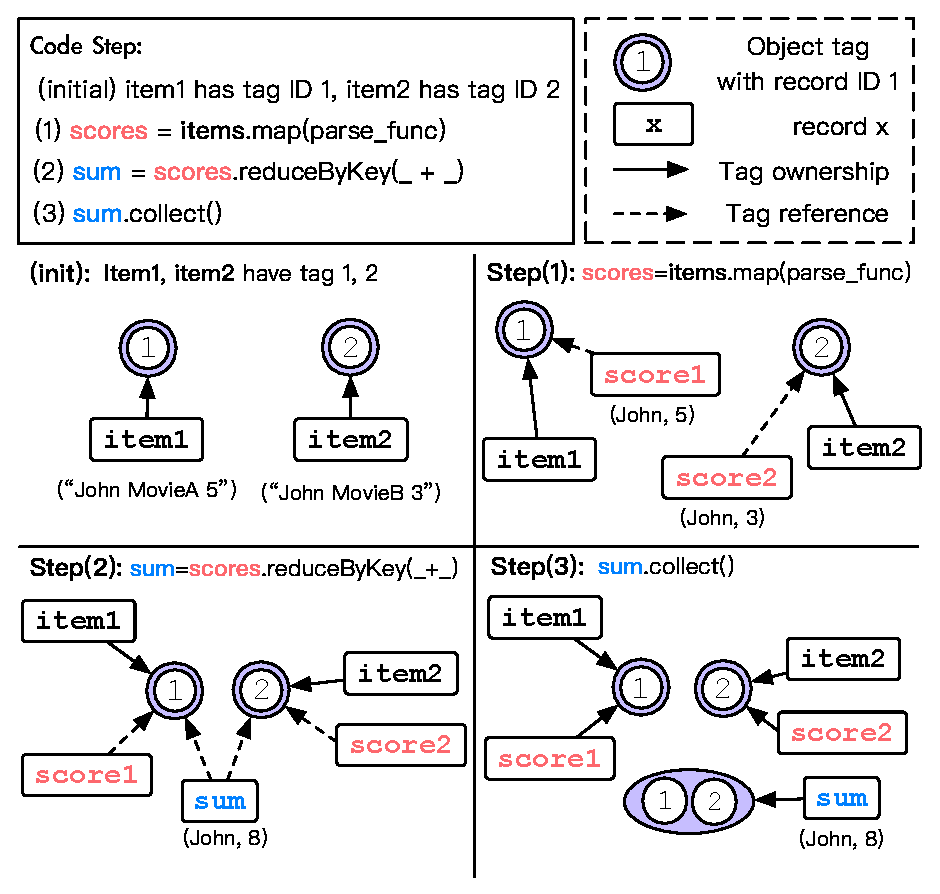
\includegraphics[width=0.4\textwidth]{figures/reference}
\caption{The Reference Propagation technique with the given code.}
\label{fig:reference}
\end{figure}
\vspace{0.3in}

\begin{figure}[h]
   \center
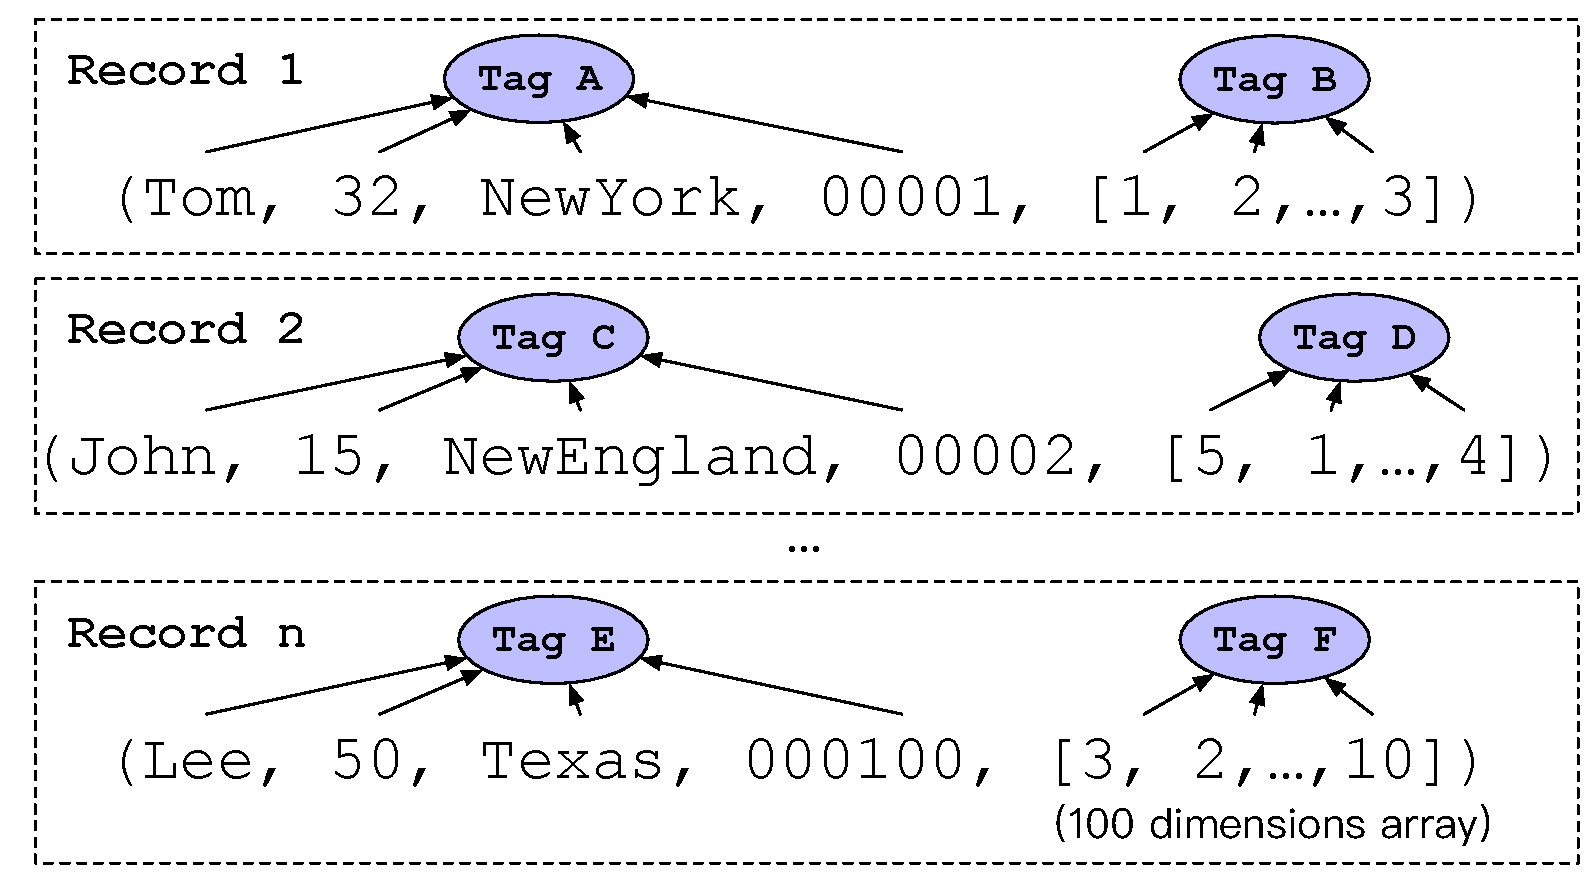
\includegraphics[width=0.4\textwidth]{figures/tagcache}
\caption{The Tag Sharing technique between fields in each record.}
\label{fig:tagcache}
\end{figure}
\vspace{0.3in}

\begin{figure}[h]
   \center
   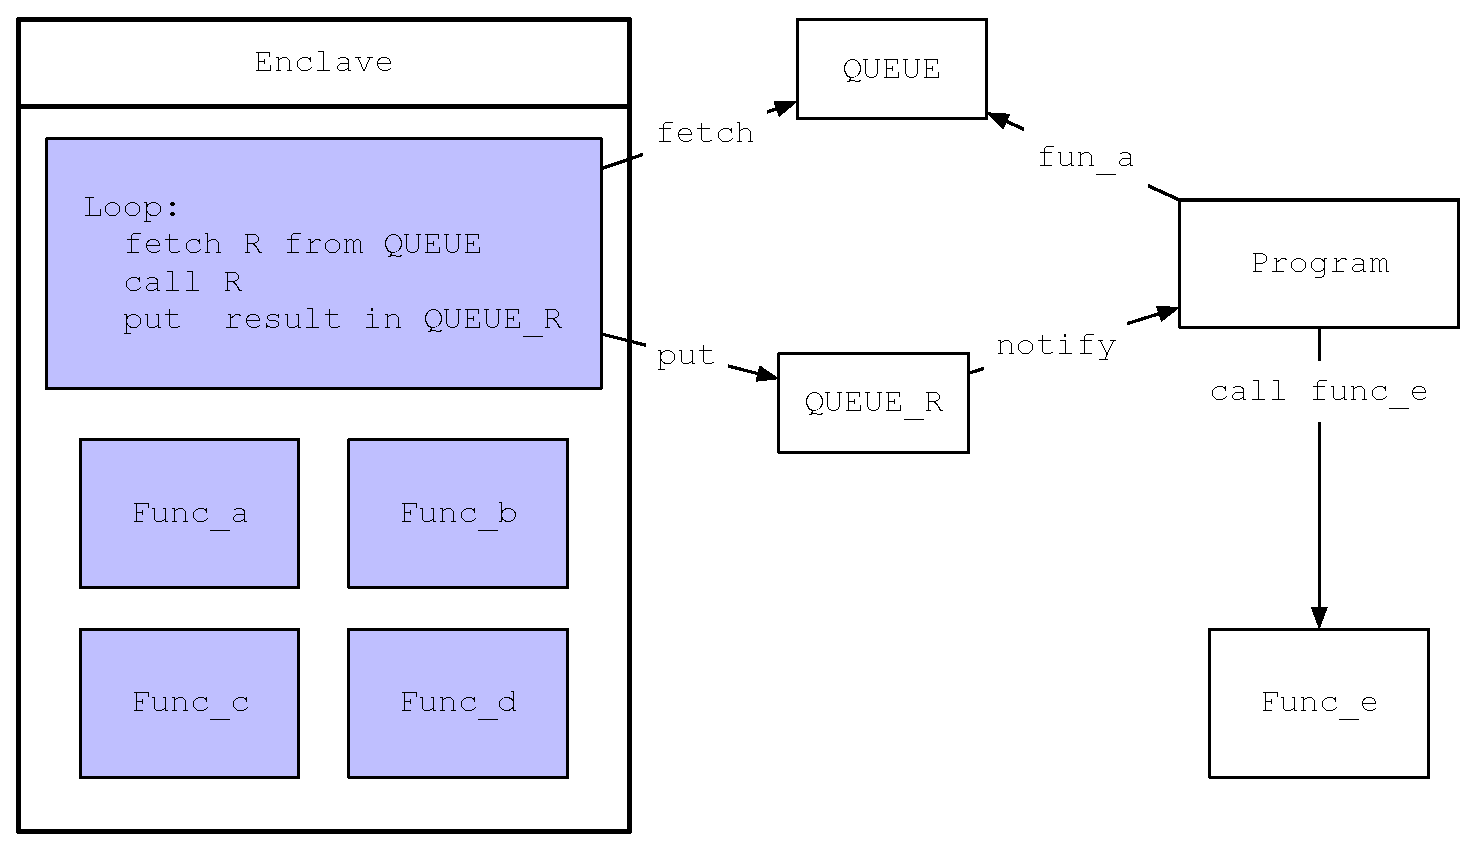
\includegraphics[width=0.4\textwidth]{figures/async_call}
 \caption{The Data-locality-aware Asynchronous Enclave (DAE) call abstraction.}
   \label{fig:async-call}
 \end{figure}

% \bibliographystyle{abbrvnat}
% \bibliography{bib/biblio}

% % \documentclass[12pt]{sosp2015}
\documentclass[12pt,inchmargins]{article}
% \usepackage[11pt,inchmargins]{sigmin}
\usepackage[T1]{fontenc}
\usepackage{tgtermes}
\usepackage{atbegshi}
%\usepackage{showframe}

\usepackage{graphics}
\usepackage{epsfig}
\usepackage{xspace}
\usepackage[nolineno,noindent,norules]{lgrind}
\usepackage{subfig,graphics,graphicx,color}
\DeclareGraphicsExtensions{.eps}


% \def\v#1{{\texttt{\fontfamily{cmtt}\fontsize{\f@size}{\f@size}\selectfont #1}}}
\let\vv\texttt

%% Title stuff.
%\newcommand{\mytitle}[0]{\textbf {Stable Multithreading: \\
%A New Paradigm for Reliable and Secure Threads}}
%\newcommand{\mykeywords}[0]{Deterministic Multithreading, Stable 
%Multithreading, Reliability, Security, Software Model Checking,
%State Space Reduction, State Machine Replication}




%% Terminology of our own internal techniques.
\newcommand{\kakute}[0]{\textsc{Kakute}\xspace}
\newcommand{\confluence}[0]{\textsc{Confluence}\xspace}
\newcommand{\pig}[0]{\textsc{Pig}\xspace}
\newcommand{\hadoop}[0]{\textsc{Hadoop}\xspace}
\newcommand{\maat}[0]{\textsc{Maat}\xspace}
\newcommand{\chref}[1]{\S\ref{#1}}
\newcommand{\lazyp}[0]{Reference Propagation\xspace}
\newcommand{\tagcache}[0]{Tag Sharing\xspace}
\newcommand{\func}[1]{\textsc{#1}}


% Objective 1
\newcommand{\appsn}[0]{4\space}
\newcommand{\appeval}[0]{seven\xspace}
\newcommand{\overheadcomp}[0]{50\%\xspace}
\newcommand{\overheadmem}[0]{1x\xspace}
\newcommand{\dagfull}[0]{Directed acyclic graph\space}
\newcommand{\timelow}[0]{60\%\space}
\newcommand{\timehigh}[0]{4.5X\space}
\newcommand{\timeavg}[0]{32.3\%\space}


%% Systems and techniques names.
% \newcommand{\xxx}[0]{\textsc{Gaia}\xspace}
\newcommand{\paxos}[0]{\textsc{Paxos}\xspace}
\newcommand{\spaxos}[0]{S-Paxos\xspace}
\newcommand{\zookeeper}{ZooKeeper\xspace}
\newcommand{\libpaxos}{libPaxos\xspace}
\newcommand{\dare}{DARE\xspace}
\newcommand{\crane}{\textsc{Crane}\xspace}
\newcommand{\falcon}{\textsc{Apus}\xspace}
\newcommand{\tripod}{\textsc{Tripod}\xspace}
\newcommand{\mesos}{\textsc{Mesos}\xspace}

\newcommand{\dmt}[0]{DMT\xspace}
\newcommand{\smt}[0]{StableMT\xspace}
\newcommand{\smr}[0]{SMR\xspace}
\newcommand{\racepro}[0]{\textsc{RacePro}\xspace}
\newcommand{\tern}[0]{\textsc{Tern}\xspace}
\newcommand{\peregrine}[0]{\textsc{Peregrine}\xspace}
\newcommand{\parrot}[0]{\textsc{Parrot}\xspace}
\newcommand{\grace}[0]{Grace\xspace}
\newcommand{\coredet}[0]{\textsc{CoreDet}\xspace}
\newcommand{\kendo}[0]{Kendo\xspace}
\newcommand{\dthreads}[0]{\textsc{DThreads}\xspace}
\newcommand{\determinator}[0]{Determinator\xspace}
\newcommand{\dbug}[0]{\textsc{dbug}\xspace}
\newcommand{\ecosys}[0]{\parrot-\dbug}
\newcommand{\ldpreload}[0]{LD\_PRELOAD\xspace}

\newcommand{\mutexlock}[0]{\texttt{pthread\_mutex\_lock}\xspace}
\newcommand{\send}[0]{\texttt{send}\xspace}
\newcommand{\accept}[0]{\texttt{accept}\xspace}
\newcommand{\connect}[0]{\texttt{connect}\xspace}
\newcommand{\recv}[0]{\texttt{recv}\xspace}
\newcommand{\sockread}[0]{\texttt{read}\xspace}
\newcommand{\close}[0]{\texttt{close}\xspace}
\newcommand{\select}[0]{\texttt{select}\xspace}
\newcommand{\poll}[0]{\texttt{poll}\xspace}
\newcommand{\epoll}[0]{\texttt{epoll}\xspace}
\newcommand{\randfunc}[0]{\texttt{rand}\xspace}
\newcommand{\srandfunc}[0]{\texttt{srand}\xspace}
\newcommand{\gettimeofday}[0]{\texttt{gettimeofday}\xspace}
\newcommand{\us}[0]{\(\mu\text{s}\)\xspace}
%\newcommand{\N}[0]{$N$\xspace}
%\newcommand{\M}[0]{$M$\xspace}
%\newcommand{\C}[0]{$C$\xspace}
%\newcommand{\timev}[0]{\texttt{T_{v}}\xspace}

%% Application names.
\newcommand{\azure}{Microsoft Azure\xspace}
\newcommand{\libsafe}{Libsafe\xspace}
\newcommand{\apache}{Apache\xspace}
\newcommand{\clamav}{ClamAV\xspace}
\newcommand{\ab}{ApacheBench\xspace}
\newcommand{\mysql}{MySQL\xspace}
\newcommand{\sysbench}{SysBench\xspace}
\newcommand{\mplayer}[0]{{MPlayer}\xspace}
\newcommand{\mencoder}[0]{\v{mencoder}\xspace}
\newcommand{\pbzip}[0]{\v{PBZip2}\xspace}
\newcommand{\aget}[0]{\v{aget}\xspace}
\newcommand{\mongoose}[0]{\v{Mongoose}\xspace}
\newcommand{\pfscan}[0]{\v{pfscan}\xspace}
\newcommand{\fft}[0]{\v{fft}\xspace}
\newcommand{\luc}[0]{\v{lu\_cb}\xspace}
\newcommand{\lun}[0]{\v{lu\_ncb}\xspace}
\newcommand{\barnes}[0]{\v{barnes}\xspace}
\newcommand{\radix}[0]{\v{radix}\xspace}
\newcommand{\radiosity}[0]{\v{radiosity}\xspace}
\newcommand{\waters}[0]{\v{water-spatial}\xspace}
\newcommand{\watern}[0]{\v{water-nsquared}\xspace}
\newcommand{\oceanncp}[0]{\v{ocean}\xspace}
\newcommand{\oceancp}[0]{\v{ocean}\xspace}
\newcommand{\ocean}[0]{\v{ocean}\xspace}
\newcommand{\fmm}[0]{\v{fmm}\xspace}
\newcommand{\volrend}[0]{\v{volrend}\xspace}
\newcommand{\cholesky}[0]{\v{cholesky}\xspace}
\newcommand{\streamcluster}[0]{\v{streamcluster}\xspace}
\newcommand{\blackscholes}[0]{\v{blackscholes}\xspace}
\newcommand{\swaptions}[0]{\v{swaptions}\xspace}
\newcommand{\bodytrack}[0]{\v{bodytrack}\xspace}
\newcommand{\bodytrackopenmp}[0]{\v{bodytrack-openmp}\xspace}
\newcommand{\ferret}[0]{\v{ferret}\xspace}
\newcommand{\dedup}[0]{\v{dedup}\xspace}
\newcommand{\raytrace}[0]{\v{raytrace}\xspace}
\newcommand{\canneal}[0]{\v{canneal}\xspace}
\newcommand{\racey}[0]{\v{racey}\xspace}
\newcommand{\freqmine}[0]{\v{freqmine}\xspace}
\newcommand{\vips}[0]{\v{vips}\xspace}
\newcommand{\xtwosixfour}[0]{\v{x264}\xspace}
\newcommand{\fluidanimate}[0]{\v{fluidanimate}\xspace}
\newcommand{\facesim}[0]{\v{facesim}\xspace}
\newcommand{\rtviewraytrace}[0]{\v{rtview\_raytrace}\xspace}
\newcommand{\wordcount}[0]{\v{word\_count}\xspace}
\newcommand{\klee}[0]{\textsc{klee}\xspace}
\newcommand{\woodpecker}[0]{\textsc{woodpecker}\xspace}
\newcommand{\splashx}[0]{\mbox{SPLASH-2x}\xspace}
\newcommand{\splash}[0]{\mbox{SPLASH-2}\xspace}
\newcommand{\parsec}[0]{\mbox{PARSEC}\xspace}
\newcommand{\phoenix}[0]{\mbox{Phoenix}\xspace}
\newcommand{\pthread}[0]{\mbox{Pthreads}\xspace}

%% Application names (continue).
\newcommand{\kmeans}[0]{\v{kmeans}\xspace}
\newcommand{\kmeanspthread}[0]{\v{kmeans-pthread}\xspace}
\newcommand{\linearregre}[0]{\v{linear-regression}\xspace}
\newcommand{\linearregrepthread}[0]{\v{linear-regression-pthread}\xspace}
\newcommand{\matrixmult}[0]{\v{matrix-multiply}\xspace}
\newcommand{\matrixmultpthread}[0]{\v{matrix-multiply-pthread}\xspace}
\newcommand{\wordcnt}[0]{\v{word-count}\xspace}
\newcommand{\wordcntpthread}[0]{\v{word-count-pthread}\xspace}
\newcommand{\stringmatch}[0]{\v{string-match}\xspace}
\newcommand{\stringmatchpthread}[0]{\v{string-match-pthread}\xspace}
\newcommand{\histogram}[0]{\v{histogram}\xspace}
\newcommand{\histogrampthread}[0]{\v{histogram-pthread}\xspace}
\newcommand{\pca}[0]{\v{pca}\xspace}
\newcommand{\pcapthread}[0]{\v{pca-pthread}\xspace}

%% Application names (continue).
\newcommand{\partition}[0]{\mbox{\v{partition}}\xspace}
\newcommand{\nthelement}[0]{\mbox{\v{nth\_element}}\xspace}
\newcommand{\partialsort}[0]{\mbox{\v{partial\_sort}}\xspace}
\newcommand{\ua}[0]{\v{ua}\xspace}
\newcommand{\is}[0]{\v{is}\xspace}
\newcommand{\npb}[0]{\mbox{NPB}\xspace}
\newcommand{\imagick}[0]{\mbox{ImageMagick}\xspace}
\newcommand{\openldap}[0]{{OpenLDAP}\xspace}
\newcommand{\redis}[0]{{Redis}\xspace}
\newcommand{\memcached}[0]{{Memcached}\xspace}
\newcommand{\bdb}[0]{{Berkeley DB}\xspace}
\newcommand{\openmp}[0]{{OpenMP}\xspace}
\newcommand{\libgomp}[0]{\v{libgomp}\xspace}
\newcommand{\vtune}[0]{\v{VTune}\xspace}

%% concurrency attack study stats.
\newcommand{\noldattacks}[0]{46\xspace}
\newcommand{\nattacks}[0]{23\xspace}

%% imagick programs
\newcommand{\convertshear}[0]{\v{convert\_shear}\xspace}
\newcommand{\montage}[0]{\v{montage}\xspace}

\newcommand{\nprog}[0]{108\xspace}
\newcommand{\nrealprog}[0]{55\xspace}
\newcommand{\nstl}[0]{33\xspace}
\newcommand{\nimagick}[0]{14\xspace}
\newcommand{\nparsec}[0]{15\xspace}
\newcommand{\nphoenix}[0]{14\xspace}
\newcommand{\nsplash}[0]{14\xspace}
\newcommand{\nnpb}[0]{10\xspace}
\newcommand{\nbenchmarks}[0]{53\xspace}
\newcommand{\ndatapartition}[0]{86\xspace}
\newcommand{\nprogadhocsync}[0]{5\xspace}
\newcommand{\nprogtimeout}[0]{5\xspace}

\newcommand{\nprognohints}[0]{18\xspace}
\newcommand{\nprogneedhints}[0]{90\xspace}
\newcommand{\nprognondethints}[0]{9\xspace}
\newcommand{\nprognondetandnetwork}[0]{11\xspace} % the UA program is excluded.
\newcommand{\nprognonondethints}[0]{99\xspace}
\newcommand{\nproglineuphints}[0]{81\xspace}
\newcommand{\nproggenericlineuphints}[0]{43\xspace}
\newcommand{\nprogspecificlineuphints}[0]{38\xspace}
\newcommand{\nlineofhints}[0]{109\xspace}
\newcommand{\nlineofcomputehints}[0]{87\xspace}
\newcommand{\nlineofnondethints}[0]{22\xspace}
\newcommand{\hintsperprog}[0]{1.2\xspace}
\newcommand{\nlineupfails}[0]{12\xspace}

%% effects of perfomance hints.
\newcommand{\genericnolineup}[0]{500\%\xspace}
\newcommand{\genericlineup}[0]{0.8\%\xspace}
\newcommand{\specificnolineup}[0]{460\%\xspace}
\newcommand{\specificlineup}[0]{19.1\%\xspace}
\newcommand{\nondetnohints}[0]{830\%\xspace}
\newcommand{\nondethints}[0]{42.1\%\xspace}
\newcommand{\overallnohints}[0]{510\%\xspace}
\newcommand{\overallhints}[0]{11.9\%\xspace}

%% our geometric mean overhead on standard workload.
\newcommand{\meanoverhead}[0]{12.7\%\xspace}
\newcommand{\meanrealoverhead}[0]{6.9\%\xspace}
\newcommand{\meanbenchoverhead}[0]{19.0\%\xspace}

%% model checking reduction.
%% nprogshrink, totally 56: 50 programs with out nondet hints, and 6 programs with network or nondet hints.
\newcommand{\shrinkscale}[0]{$10^{6}$--$10^{19734}$\xspace}
\newcommand{\nprogshrink}[0]{56\xspace}
\newcommand{\nprognondetshrink}[0]{5\xspace}
\newcommand{\nprogverifiedxxx}[0]{99\xspace}
\newcommand{\nprogverifieddbug}[0]{43\xspace}

%% overheads in comparison table.
\newcommand{\nprogcompared}[0]{25\xspace}
\newcommand{\xxxcompoverhead}[0]{11.8\%\xspace}
\newcommand{\dthreadssyncoverhead}[0]{150.0\%\xspace}
\newcommand{\dthreadssyncoverheadnoflui}[0]{112.5\%\xspace}
%\newcommand{\dthreadsoverhead}[0]{1,173\%\xspace}
\newcommand{\dthreadsexampleoverhead}[0]{7.7$\times$\xspace}
\newcommand{\coredetoverhead}[0]{115.1\%\xspace}
\newcommand{\overeach}[0]{10$\times$\xspace}
\newcommand{\overcombined}[0]{4$\times$\xspace}

% Stats
\newcommand{\fasterDARElow}[0]{7.9\%\xspace}
\newcommand{\fasterDARE}[0]{3.3X\xspace}
\newcommand{\xxxlatencythree}[0]{8.2\xspace}
\newcommand{\xxxlatencyonezerofive}[0]{31.6\xspace}

\newcommand{\comptradlow}[0]{32.3X\xspace} % TBD
\newcommand{\comptradhigh}[0]{85.8X\xspace} % TBD

\newcommand{\tradlatencyincreaselow}[0]{30.3\%\xspace} % TBD
\newcommand{\tradlatencyincreasehigh}[0]{156.8\%\xspace} % TBD
\newcommand{\systemcostlow}[0]{36.5\%\xspace} % TBD
\newcommand{\systemcosthigh}[0]{63.7\%\xspace} % TBD
\newcommand{\xxxscalability}[0]{3.8x\xspace} % TBD
\newcommand{\darescalability}[0]{11.7x\xspace} % TBD

% Tripod result.
\newcommand{\tputoverhead}[0]{3.22\%\xspace}
\newcommand{\latencyoverhead}[0]{3.31\%\xspace}

\newcommand{\eg}{{e.g.}}
\newcommand{\ie}{{i.e.}}
\newcommand{\etc}{{etc}}
\newcommand{\para}[1]{\vspace{.00in}\noindent{\bf #1}}
\newcommand{\wrt}{{w.r.t. }}
\newcommand{\cf}{{cf. }}
\newcommand{\vs}{{vs.}\xspace}

\newcommand{\github}[0]{\url{github.com/columbia/smt-mc}}


%% Reference stuff.
\usepackage[square,comma,numbers,sort]{natbib}
\usepackage{hypernat}
\usepackage{hyperref}
\hypersetup{
  colorlinks=false,
  pdfborder={0 0 0},
  %pdftitle={\mytitle},
  %pdfkeywords={\mykeywords},
  bookmarksnumbered,
  pdfstartview={FitH},
  urlcolor=cyan,
  pdfpagelabels=true,
  pdfdisplaydoctitle=true,
}



% <http://psl.cs.columbia.edu/phdczar/proposal.html>:
%
% The standard departmental thesis proposal format is the following:
%        30 pages
%        12 point type
%        1 inch margins all around = 6.5   inch column
%        (Total:  30 * 6.5   = 195 page-inches)
%
% For letter-size paper: 8.5 in x 11 in
% Latex Origin is 1''/1'', so measurements are relative to this.

\topmargin      0.0in
\headheight     0.0in
\headsep        0.0in
\oddsidemargin  0.0in
\evensidemargin 0.0in
\textheight     9.0in
\textwidth      6.5in

\title{
{Doctoral Thesis Proposal} \\
~\\
\bf \mytitle}
\author{ {Heming Cui}  \\
Department of Computer Science \\
Columbia University\\
{\small heming@cs.columbia.edu} \\
}
\date{\today}

\begin{document}
\pagestyle{plain}
\pagenumbering{roman}

\cleardoublepage
\pagenumbering{arabic}

\vspace{-.15in}\section{Research Background} 
\label{sec:background}\vspace{-.075in}


This section introduces the background of big-data 
frameworks (\S\ref{sec:bigdata}), sofware-based privacy techniques  
(\S\ref{sec:dft}), hardware-based privacy techniques (\S\ref{sec:sgx}), 
motivation of objectives (\S\ref{sec:motivation}), and related work 
(\S\ref{sec:others-work} and \S\ref{sec:my-work}).


\vspace{-.15in}\subsection{Big-data Computing Frameworks} 
\label{sec:bigdata}\vspace{-.075in}

Big-data frameworks (\eg Spark~\cite{nsdi12:spark}, 
DryadLINQ~\cite{osdi08:dryad}, MapReduce \cite{mapreduce}) are popular for 
computations on tremendous amounts of data. These frameworks provide 
self-defined functions (\eg, map and reduce) to let computation providors 
write their algorithms to perform queries or transformations on data, and these 
frameworks automatically apply the functions on the data stored across 
computers in parallel. To exchange intermediate results across hosts, shuffles 
operations are often invoked and sometimes they are performance bottlenecks in 
big-data frameworks. For instance, Spark~\cite{nsdi12:spark} has intensive data 
shuffling beteen its map and reduce stages.

% Many-to-many transformations (\eg \func{groupByKey}, \func{join}
% and \func{aggregateByKey}) are prevalent in these frameworks. Each many-to-many
% transformation takes many input records and generates many output records.
% Given an output record, extant data provenance 
% techniques~\cite{icse16:bigdebug,vldb15:titian,vldb16:output}, which track the 
% sequence of transformation operations for data records and can infer the input 
% records on a given output record, will
% report all input records going through this transformation, including many
% irrelevant input records that generate other output records.


To avoid excessive computation, many DISC systems adopt the lazy transformation 
approach~\cite{pig:vldb08,nsdi12:spark,osdi08:dryad}. Spark uses lazy 
transformations (\eg \func{map}) for efficiency, and calls to these 
transformations only create a new data structure called \func{RDD} with 
\func{lineage} (the sequence of transformation operations for a data record).
The real transformations are only triggered when collecting operations (\eg 
\func{collect}, \func{count}) are called. These collecting operations trigger 
transformations along lineages, where unnecessary computations are avoided. 
\textbf{Objective 1} (\chref{sec:kakute}) leverages the lazy transformation
feature in big-data frameworks to develop the new \lazyp technique.

\vspace{-.15in}\subsection{Software-based Privacy Techniques}
\label{sec:dft}\vspace{-.075in}

Data Flow Tracking (DFT) is a mandatory access control technique for preventing 
sensitive information leakage~\cite{dawn05:taint}. DFT attaches a tag to a 
variable (or object), and this tag will propagate throughout the computation at 
runtime. For example, a variable-level dataflow tracking will involve 
combinations of tags of two variables in each instruction, using an IOR 
operation. Different granularities of computation may incur different levels of 
computation overhead. Lower level (\eg byte-level) tracking will consume a lot 
of resources, as each byte of data in an DFT system has its own 
tags~\cite{libdft:vee12}. DFT has been applied to various areas, such as 
preventing sensitive information 
(\eg GPS data and contacts) leakage in cellphone~\cite{taintdroid:osdi10, 
cleanos:osdi12}, providing secure web services~\cite{cloudfence:raid13} and 
server programs~\cite{libdft:vee12}. To the best of our knowledge, no 
DFT system exists for big-data computing.
 
% Multiple research has been focusing on efficiency and applications of DFT.
% Shadowreplica~\cite{shadowreplica:ccs13} proposed to make use of the multicore 
% resources while SHIFT~\cite{hardwardtaint:isca08} suggests accelerating 
% dataflow tracking with hardware support. Several 
% research~\cite{mit07:coverage,fse12:dtam} adopts DFT for providing 
% debugging primitives to improve software reliability.


Complimentary to DFT, statistical techniques allow the aggregration of 
sensitive data while preserving the privacy of any individual one. These 
statistical techniques include k\-anonymization 
methods~\cite{kanonymity,icde06:ldiversity} or
differential privacy~\cite{gupt:sigmod12, pinq:sigmod09,airavat:nsdi10}, which 
enforce statistical bounds to prevent individual information leakage.
% Therefore, third-parties can
% not get sensitive data with different queries.

However, these statistical techniques are either not secure (k\-anonymization) 
or suffering from great losses of accuracy (differential privacy). A recent
work~\cite{differentialresult:vldb15} reported more than 30\% losses of accuracy 
when the security guarantee is high (the probability of leakages is low). In 
such case, a simple KMeans program will return centroids far from the accurate 
ones, and the accuracy loss rate is much larger than the training error rate 
which is several percents in practice. Overall, despite much effort, existing 
differential privacy techniques can only favor privacy or utility of results, 
but not both, and key reason is that these techniques lack a precise tracking 
of how sensitive data fields flow to query results, so they have to take a 
coarse-grained approach, which conservatively adds noise to all fields and 
records.


In practice, only some fields in a data record may be sensitive and it is too 
rigorous to make all fields inaccurate. Moreover, different data records may 
have various security levels. For example, in an Taobao order record 
$\langle$\v{time}, \v{userId}, \v{productID}$\rangle$, the \v{userId} field is 
sensitive and it must not be leaked, and different owners of movie rating 
records may demand different levels of protection for their 
data. \textbf{Objective 2} (\chref{sec:obj2}) 
proposes a novel fine-grained differential privacy technique, which combines  
the strengths of DFT and differential privacy.
% 4. They are not accurate and per-record, only some field are sensitive



\vspace{-.15in}\subsection{Hardware-based Privacy Techniques}
\label{sec:sgx}\vspace{-.075in}

Trusted Execution Environment (TEE) is a promising technique that
protects computation on cloud even through the operating system is
compromised. The program is running in a secure environment, and memory can not
be seen by malicious parties. For example, Intel-SGX~\cite{intel-sgx} runs 
programs
in a enclave, which is protected and can not be see by the system.

However, running programs in a enclave needs modifications to the original
programs, which needs a great effort and is error-prone. Recent
work~\cite{securekeeper,opaque:nsdi17} run Zookeeper and SparkSQL in enclaves,
and both of them rewrote codes running in enclaves using C++.
BigMatrix~\cite{bigmatrix:ccs17} proposes a secure and oblivious vectorization
abstraction for Python, but it also needs modifications to the original 
programs.
These methods causes two problems. First, modifications are necessary to run
programs in enclaves. Second, running C++ in JVM breaks the protections
provided Java.

\vspace{-.15in}\subsection{Motivation of objectives} 
\label{sec:motivation}\vspace{-.075in}
TBD.

\subsection{Related work by others} 
\label{sec:others-work}\vspace{-.075in}

\para{Computing on encrypted data}. Homomorphic 
encryption~\cite{fullmomo:stoc09,paillier,elgamal} is a
technique for performing computations on encryted data in untrusted 
environments. Homomorphic encryption contain two kinds: Fully 
homomorphic encryption (FHE) and partial 
homomorphic encryption.
Partial homomorphic encryption (\eg{} Additive Homomorphic 
Encryption~\cite{paillier})
incurs a much lower overhead compared with FHE. A evaluation~\cite{homo:eval} on
FHE shows a $10e9$ slowdown, which is acceptable in practice.
Systems that adopts PHE (\eg{} Monomi~\cite{monomi:vldb13},
Crypsis~\cite{crypsis:hotcloud14}, CryptDB~\cite{cryptdb:sosp11},
MrCrypt~\cite{mrcrypt:oospsla14})
reports a much better overhead, but it has limited expressiveness
(\eg{} SQL operators) and requires extra trusted servers for computations.
Seabed~\cite{seabed:osdi16} proposes asymmetric encryption schemes and reduces 
performance overhead
incur by AHE, but it still has limited expressiveness.

\subsection{Hardware-based Privacy-preserving Analytic}
Intel SGX is a promising technique to provide privacy-preserving analytic
in public clouds. Compared with software-based solutions, hardware-based 
solutions
incurs much lower overhead. TrustedDB~\cite{trusteddb:sigmod11} is a
hardware-based secure database.
VC3~\cite{vc3:sp15} proposes a secure distributed analytic platform
with read-write validations on Mapreduce~\cite{mapreduce}. 
Opaque~\cite{opaque:nsdi17}
supports secure and oblivious SQL operators on 
SparkSQL~\cite{sparksql:sigmod15}.
However, all these systems have limited expressiveness (\eg SQL operators), and
VC3 even needs to rewrite the program with C++. A recent 
work~\cite{oblivious:security16} proposes a oblivious machine leaning
framework on trusted processors.
BigMatrix~\cite{bigmatrix:ccs17} proposes an oblivious and secure vectorization
abstraction on python, but it has limited expressiveness and it needs to
rewrite the original program with this new abstraction.
Although BigMatrix provides guideline for
writing a oblivious program, but it would be a time-consuming and error-prone
process.

\vspace{-.15in}\subsection{Related work by the PI and co-I} 
\label{sec:my-work}\vspace{-.075in}
% 
% First emphasis debugging experience on concurrency. Program analysis.
% Then mention security exploits found in Woodpecker.
% Then mention runtime systems.

The PI is an expert on secure and reliable distributed 
systems~\cite{smt:cacm, cui:tern:osdi10, peregrine:sosp11,
parrot:sosp13, crane:sosp15, tripod:apsys16, kakute:acsac17, 
confluence:tpds17}. The PI's works are published in top conferences on systems 
(OSDI, SOSP, SOCC, TPDS, and ACSAC) and programming languages (PLDI and ASPLOS). 
The co-I is an expert on high-performance 
computing~\cite{powerrock,hwang,jessica,cheung,khokhar}, fault-tolerance~\cite{ 
sheng,shengdi1}, and VMs~\cite{rhymes,shengdi,jessica2}. The 
co-I's works are published in top systems conferences (Cluster '02, SC '13, 
and ICPADS '14) and journals (JPDC '00, TPDS '13, IEEE Tran. Computers '14). As 
preliminary works for this proposal, the PI and co-I have developed 
Kakute~\cite{kakute:acsac17} and TPDS~\cite{confluence:tpds17} (parts of 
\textbf{Objective 1}). 




\section{Research Plan and Methodology} \label{sec:rep}

TBD

\subsection{\xxx Architecture Design} \label{sec:rep-arch}

TBD





% \pagebreak

\newpage
\AtBeginShipout{%
\AtBeginShipoutDiscard
}

\bibliographystyle{abbrvnat}
\bibliography{bib/biblio}

\end{document}


     %% watch out for the same name

\end{document} 
